\documentclass[tikz, border=5pt]{standalone}

% --- TIKZ GRAPHICS SETUP ---
\usepackage{tikz}
\usepackage{xcolor}
\usetikzlibrary{arrows.meta, positioning, calc}
\definecolor{Garnet}{HTML}{73000A}
\definecolor{Gray10}{gray}{0.10}
\definecolor{Gray30}{gray}{0.30}
\definecolor{Gray50}{gray}{0.50}
\definecolor{Gray70}{gray}{0.70}
\definecolor{Gray90}{gray}{0.90}

\begin{document}

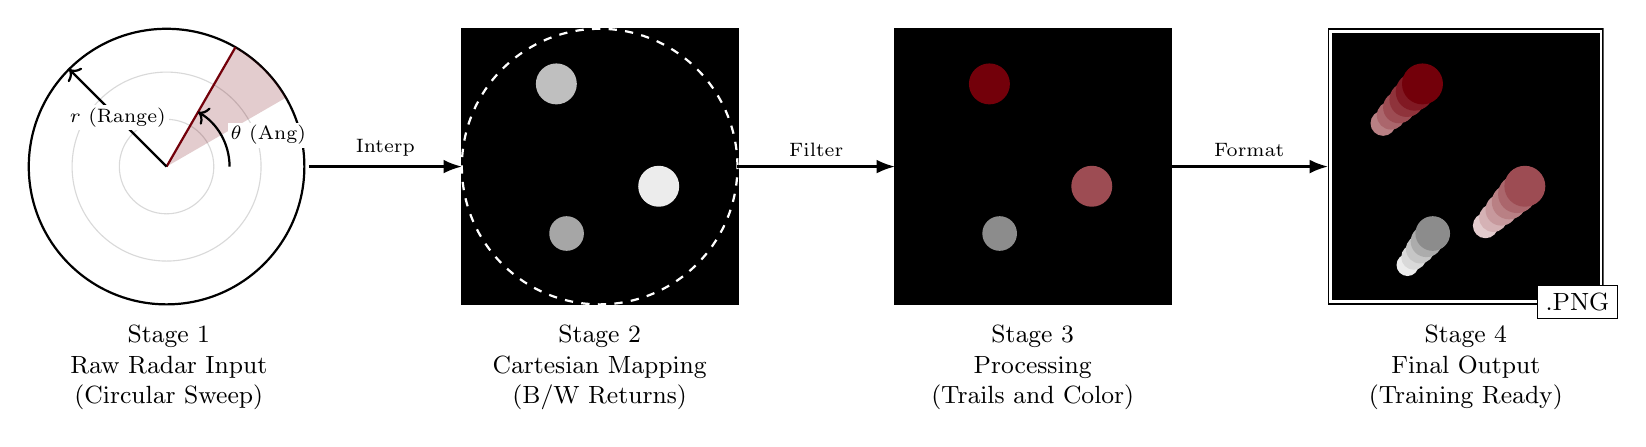
\begin{tikzpicture}[
    stage_label/.style={
        text width=3cm,
        align=center,
        font=\small,
        color=black
    },
    arrow_line/.style={
        ->, 
        >=Latex, 
        thick, 
        color=black, 
        text=black
    }
]

% =========================
% STAGE 1
% =========================
\begin{scope}[local bounding box=stage1]
    % Circular radar plot
    \draw[draw=black, thick, fill=white] (0,0) circle (1.75);
    \draw[draw=black, gray!30, thin] (0,0) circle (0.6);
    \draw[draw=black, gray!30, thin] (0,0) circle (1.2);

    % Radial line and sector
    \draw[draw=black, Garnet, thick] (0,0) -- (60:1.75);
    \fill[Garnet, opacity=0.2]
        (0,0) -- (60:1.75) arc (60:30:1.75) -- cycle;

    % Range arrow
    \draw[draw=black, ->, thick]
        (0,0) -- (135:1.75)
        node[midway, fill=white, inner sep=1pt, font=\scriptsize]
        {$r$ (Range)};

    % Angle arc
    \draw[draw=black, ->, thick]
        (0.8,0) arc (0:60:0.8)
        node[midway, right=2pt, fill=white, inner sep=1pt, font=\scriptsize]
        {$\theta$ (Ang)};
\end{scope}

\node[stage_label, anchor=north]
    at ($(stage1.south)+(0,-0.15)$)
    {Stage 1\\Raw Radar Input\\(Circular Sweep)};

% =========================
% STAGE 2
% =========================
\begin{scope}[shift={(5.5,0)}, local bounding box=stage2]
    % Cartesian mapping box
    \draw[draw=black, thick, fill=black] (-1.75,-1.75) rectangle (1.75,1.75);
    \draw[draw=black, thick, dashed, white] (0,0) circle (1.75);

    \begin{scope}
        \clip (0,0) circle (1.75);
        \fill[gray!50] (-0.55,1.05) circle (0.26);
        \fill[gray!15] (0.75,-0.25) circle (0.26);
        \fill[gray!70] (-0.42,-0.85) circle (0.22);
    \end{scope}
\end{scope}

\node[stage_label, anchor=north]
    at ($(stage2.south)+(0,-0.15)$)
    {Stage 2\\Cartesian Mapping\\(B/W Returns)};

% =========================
% STAGE 3
% =========================
\begin{scope}[shift={(11,0)}, local bounding box=stage3]
    % Processing box with garnet accent
    \draw[draw=black, thick, fill=black] (-1.75,-1.75) rectangle (1.75,1.75);
    \begin{scope}
        \clip (-1.75,-1.75) rectangle (1.75,1.75);
        \fill[Garnet] (-0.55,1.05) circle (0.26);
        \fill[Garnet!70] (0.75,-0.25) circle (0.26);
        \fill[gray!90] (-0.42,-0.85) circle (0.22);
    \end{scope}
\end{scope}

\node[stage_label, anchor=north]
    at ($(stage3.south)+(0,-0.15)$)
    {Stage 3\\Processing\\(Trails and Color)};

% =========================
% STAGE 4
% =========================
\begin{scope}[shift={(16.5,0)}, local bounding box=stage4]
    \clip (-1.75,-1.75) rectangle (1.75,1.75);
    \draw[draw=black, thick, fill=white] (-1.75,-1.75) rectangle (1.75,1.75);

    \fill[black] (-1.7,-1.7) rectangle (1.7,1.7);

    % Trails - using garnet and gray variations
    \fill[Garnet!50] (-1.05,0.55) circle (0.16);
    \fill[Garnet!60] (-0.95,0.65) circle (0.18);
    \fill[Garnet!70] (-0.85,0.75) circle (0.20);
    \fill[Garnet!80] (-0.75,0.85) circle (0.22);
    \fill[Garnet!90] (-0.65,0.95) circle (0.24);
    \fill[Garnet] (-0.55,1.05) circle (0.26);

    % Second trail using gray variations
    \fill[Garnet!20] (0.25,-0.75) circle (0.16);
    \fill[Garnet!30] (0.35,-0.65) circle (0.18);
    \fill[Garnet!40] (0.45,-0.55) circle (0.20);
    \fill[Garnet!50] (0.55,-0.45) circle (0.22);
    \fill[Garnet!60] (0.65,-0.35) circle (0.24);
    \fill[Garnet!70] (0.75,-0.25) circle (0.26);

    % Third trail using gray variations
    \fill[gray!15] (-0.74,-1.25) circle (0.14);
    \fill[gray!30] (-0.66,-1.15) circle (0.16);
    \fill[gray!45] (-0.58,-1.05) circle (0.18);
    \fill[gray!65] (-0.50,-0.95) circle (0.20);
    \fill[gray!90] (-0.42,-0.85) circle (0.22);
\end{scope}

\node[stage_label, anchor=north]
    at ($(stage4.south)+(0,-0.15)$)
    {Stage 4\\Final Output\\(Training Ready)};

\node[draw=black, fill=white, inner sep=3pt, anchor=north west, font=\small\color{black}]
    at (17.4,-1.5) {.PNG};

% =========================
% ARROWS
% =========================
\draw[arrow_line] (stage1.east) -- (stage2.west)
    node[midway, above, font=\scriptsize] {Interp};
\draw[arrow_line] (stage2.east) -- (stage3.west)
    node[midway, above, font=\scriptsize] {Filter};
\draw[arrow_line] (stage3.east) -- (stage4.west)
    node[midway, above, font=\scriptsize] {Format};

\end{tikzpicture}

\end{document}